\chapter{Architectural Design}
\section{Overview: high-level components and interactions}\label{sec: overview}
This section provides an overview of the system's architectural components and their interactions.

\begin{figure}[h]
    \centering
    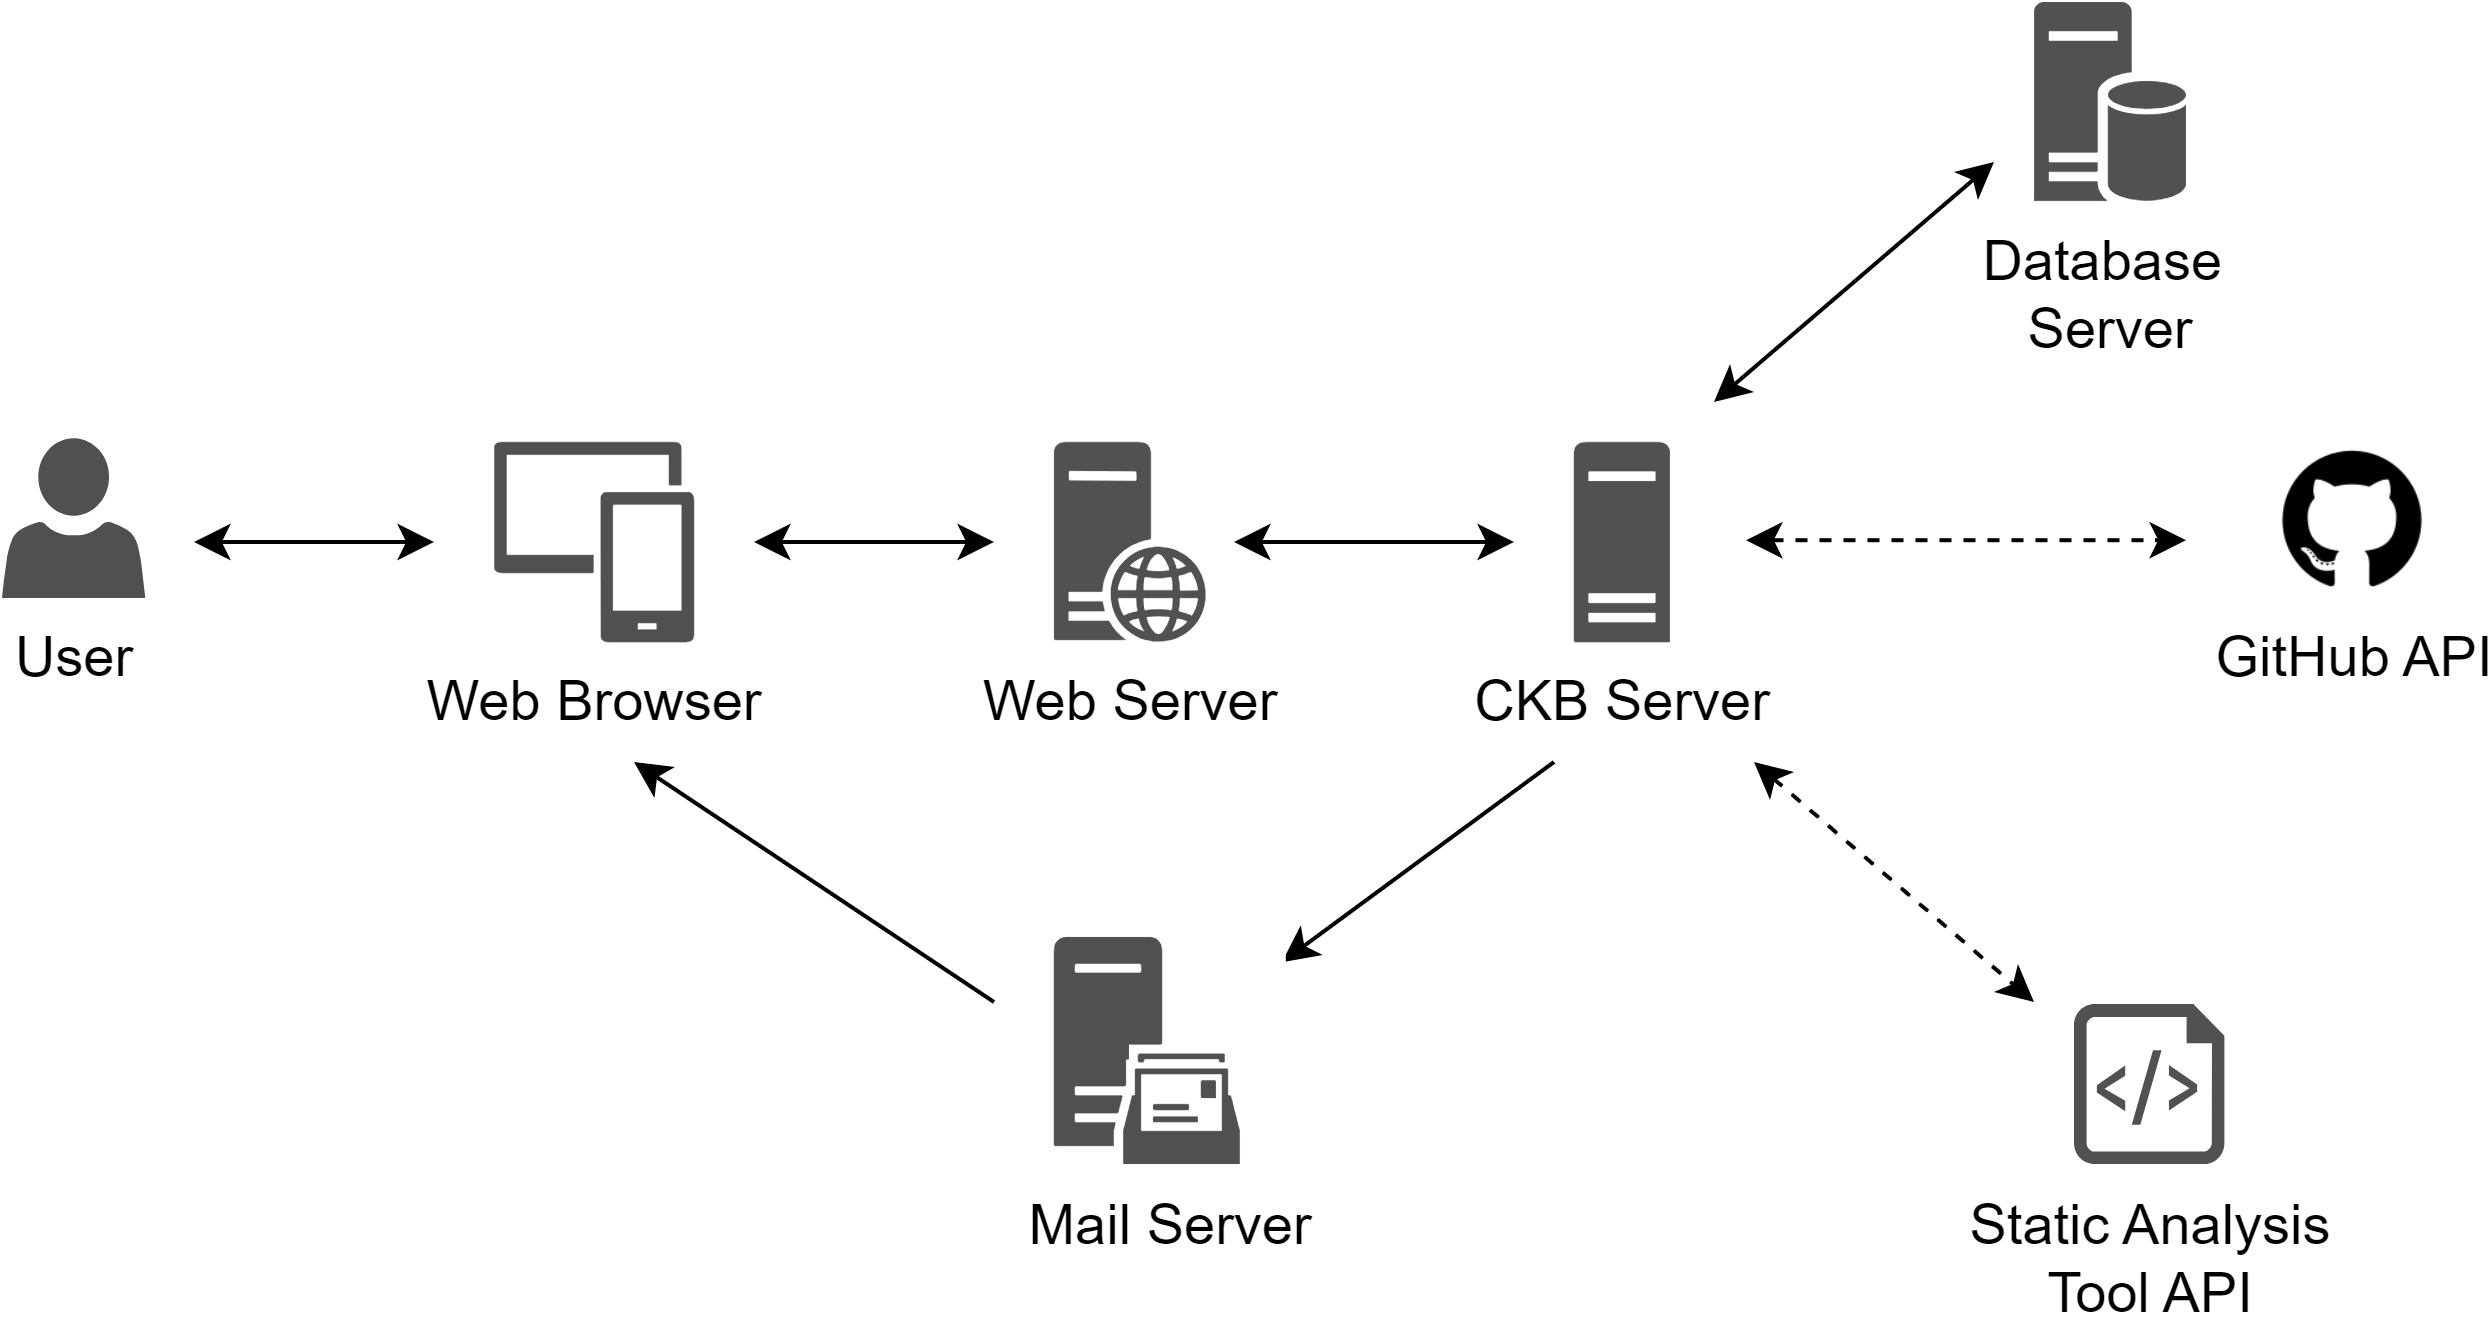
\includegraphics[width=\linewidth]{images/hl-system.png}
    \caption{CKB system overview}
    \label{fig:CKBoverview}
\end{figure}

The CKB system will be developed using the client-server paradigm:
\begin{itemize}
    \item Server side:
    \begin{itemize}
        \item Web Server: used to communicate with web browsers.
        \item CKB Server: where all the logic is located. It communicates with all other server and external tool and API. It is the central point of the system.
        \item Database Server: where all information are located.
        \item Mail Server: used to send all notifications to the users.
        \item GitHub API: used by the system to detect new push in the forked repository of the battles.
        \item Static analysis tool: used by the system to retrieve the quality level of the student's sources, in order to perform the automatic evaluation. 
    \end{itemize}
    \item Client side:
    \begin{itemize}
        \item Web browser: used by all users in order to enter the CKB website.
    \end{itemize}
\end{itemize}

The application will be developed on a three-tiered architecture where the layers (presentation, application, data) are divided into three different tiers. \newline
The client tier is responsible only of the presentation layer, therefore a thin-client has been adopted since the required client-side functionality are limited. The application tier is responsible of the application layer, it receives the request from the clients and handles them. It communicates with the data tier that is responsible of the data layer, it is able to access the data in the database. \newline
Further details on the system components and their interactions will be explained in detail in the following sections.
\clearpage

\section{Component view}
In the following section it is show the component view of the entire system, as well as all internal and external interactions. \newline
In figure \ref{fig:comp-hl} is represented all the component and the external interactions. Furthermore, in figure \ref{fig:comp-CKBserver} is represented in detail the internal structure of the CKB server, which contains the business logic of the system.

\begin{figure}[h]
    \centering
    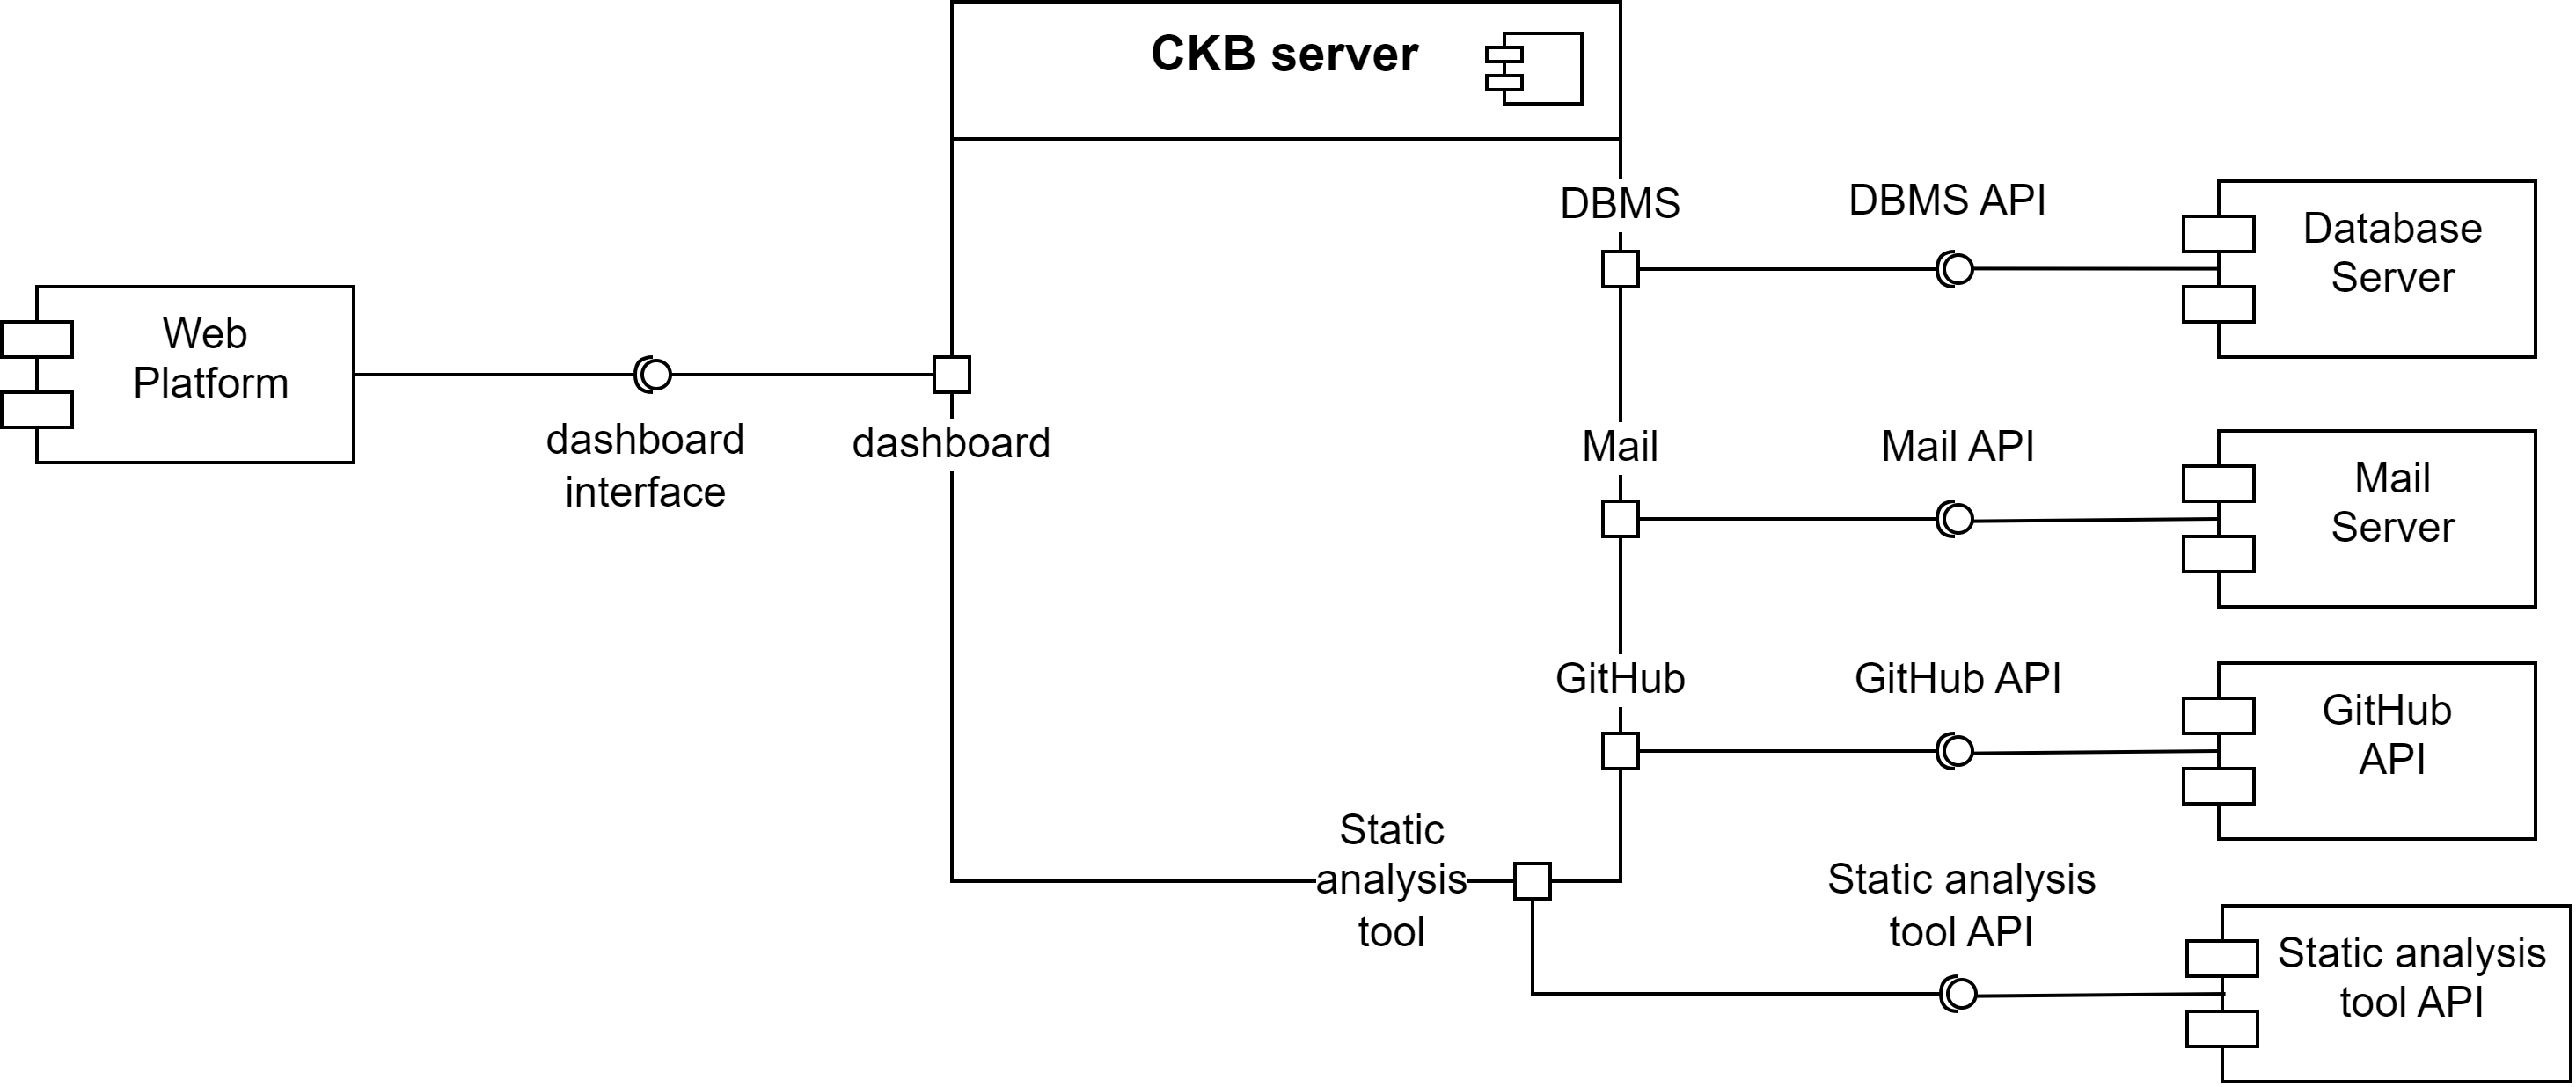
\includegraphics[width=\textwidth]{images/component-hl.png}
    \caption{Component diagram}
    \label{fig:comp-hl}
\end{figure}

The external components of the CKB system represented in figure \ref{fig:comp-hl} are:
\begin{itemize}
    \item Web platform: is the presentation layer of the website that allow all users to use the CKB functionalities.
    \item Mail service: used by the CKB system to send notification to all registered users when needed.
    \item Database: where all the data are stored. It communicate with the DBMS running on the database.
    \item GitHub API: it trigger the CKB system when there is a new push in any forked repository of a battle, in order to perform the automatic evaluation. 
    \item Static analysis tool API: it is used by the CKB system in order to retrieve the quality level of the student's sources, in order to perform the automatic evaluation. 
\end{itemize}

The internal components of the CKB server represented in figure \ref{fig:comp-CKBserver} are:
\begin{itemize}
    \item Dashboard manager: handles all the interfaces offered in the web platform and it is in charge of providing the right interface to each user.
    \item Tournament manager: handles the main features that allows educators to create and manage a tournament. It also manages all the tournament rankings.
    \item Battle manager: handles the main features that allows educators to create and manage a battle, and students to manage their teams. It also manages all the battle real-time rankings.
    \item User access manager: handles the log in and sign up functions. It also manages all students profile.
    \item Model: almost all components interacts with the model, since it is the entry point to the data stored in the database.
    \item Entity manager: it deals with all the data management needed by the system.
    \item Mail manager: interfaces with the Mail API to send notifications via email to all users.
    \item Automatic evaluation manager: it deals with both the GitHub API and the static analysis tool API, in order to modify the real-time rank of a battle.
\end{itemize}

\begin{figure}[h]
    \centering
    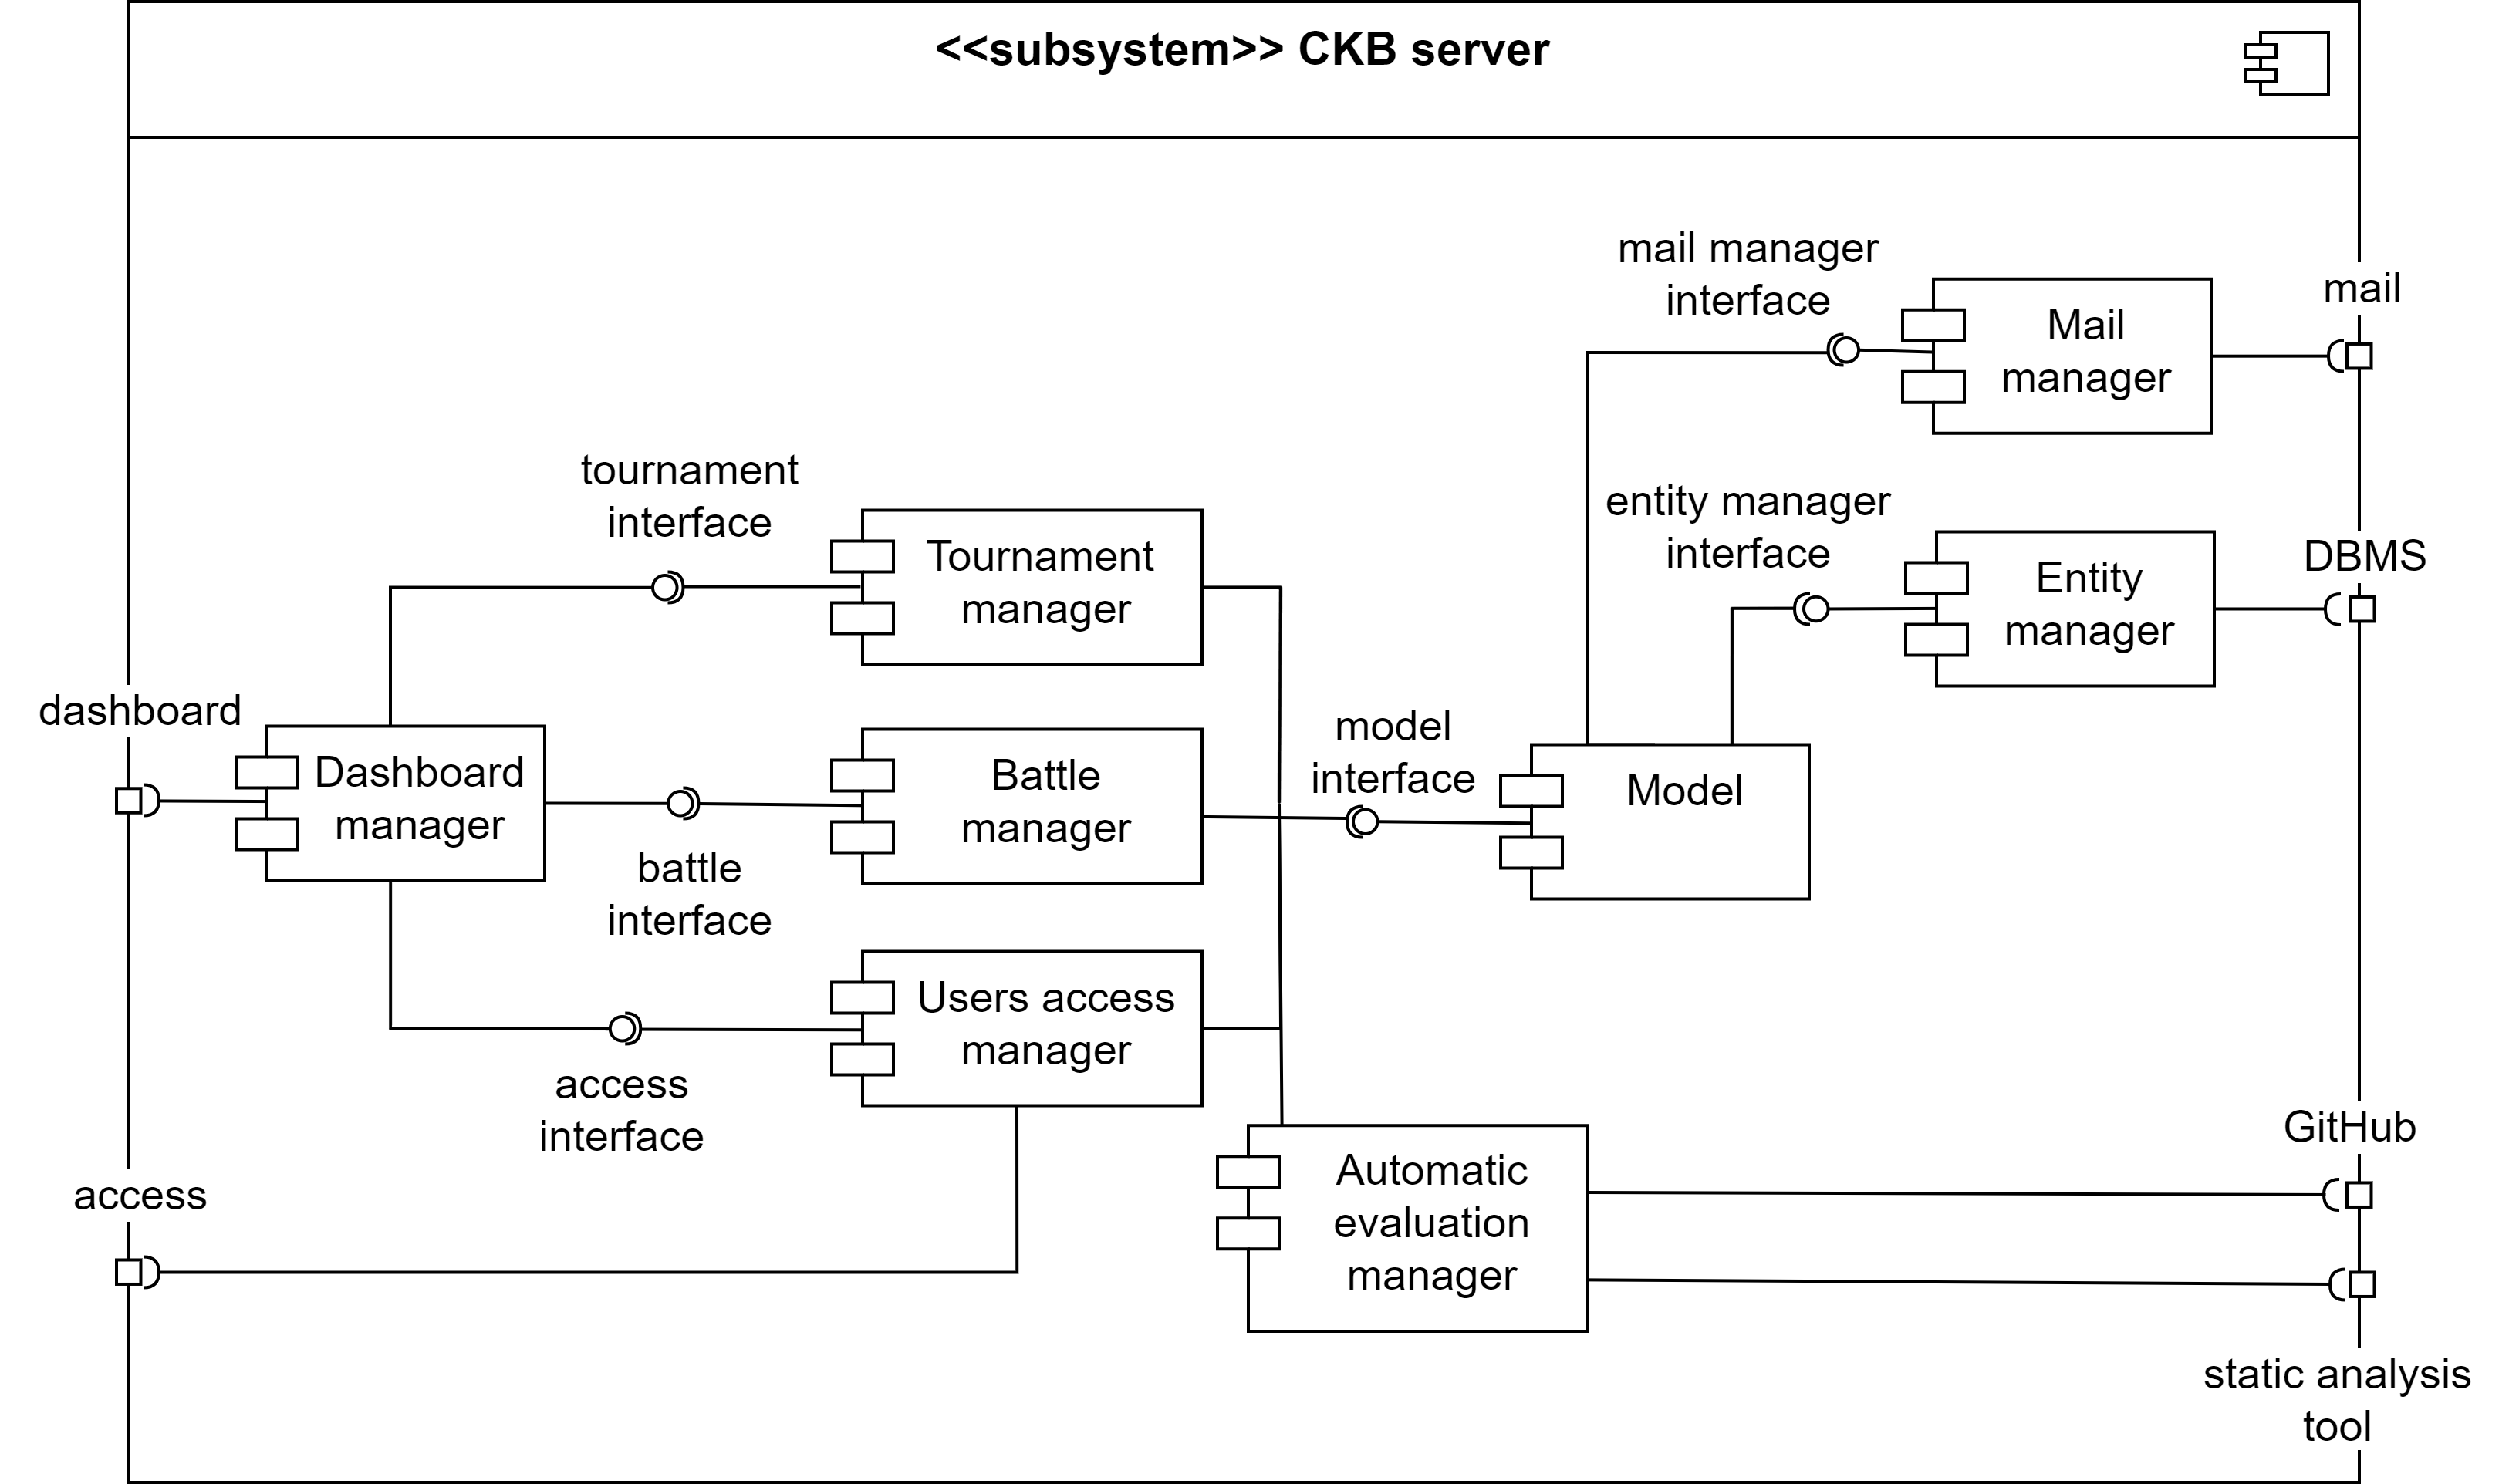
\includegraphics[width=\textwidth]{images/component-CKBserver.png}
    \caption{Component CKB server diagram}
    \label{fig:comp-CKBserver}
\end{figure}

A further explanation of the relevant internal components follows.

\subsubsection*{Dashboard manager}
\subsubsection*{Tournament manager}
\subsubsection*{Battle manager}
\subsubsection*{User access manager}
\subsubsection*{Automatic evaluation manager}

\clearpage
\section{Deployment view}\label{sec: deployment}
As previously stated in section \ref{sec: overview} the CKB system will be implemented through a three-tier architecture as shown in figure \ref{fig:deployment}. \newline
The three-tired architecture is a well-established software application architecture that organizes the system into three logical and physical computing layers:
\begin{itemize}
    \item \textbf{Presentation layer/tier}: it is the user interface where the user interacts with the application. It communicates with the application layer in order to retrieve all necessary information requested by the user. Its main purpose is to display information and collect information from the user.
    \item \textbf{Application layer/tier}: it manages all system functionalities. All information collected in the application layer are processed using a specific business logic. It communicates with the data layer in order to store, delete or modify useful data.
    \item \textbf{Data layer/tier}: it includes the database of the system and all necessary mechanism to extract and evaluate data.
\end{itemize}
\begin{figure}[h]
    \centering 
    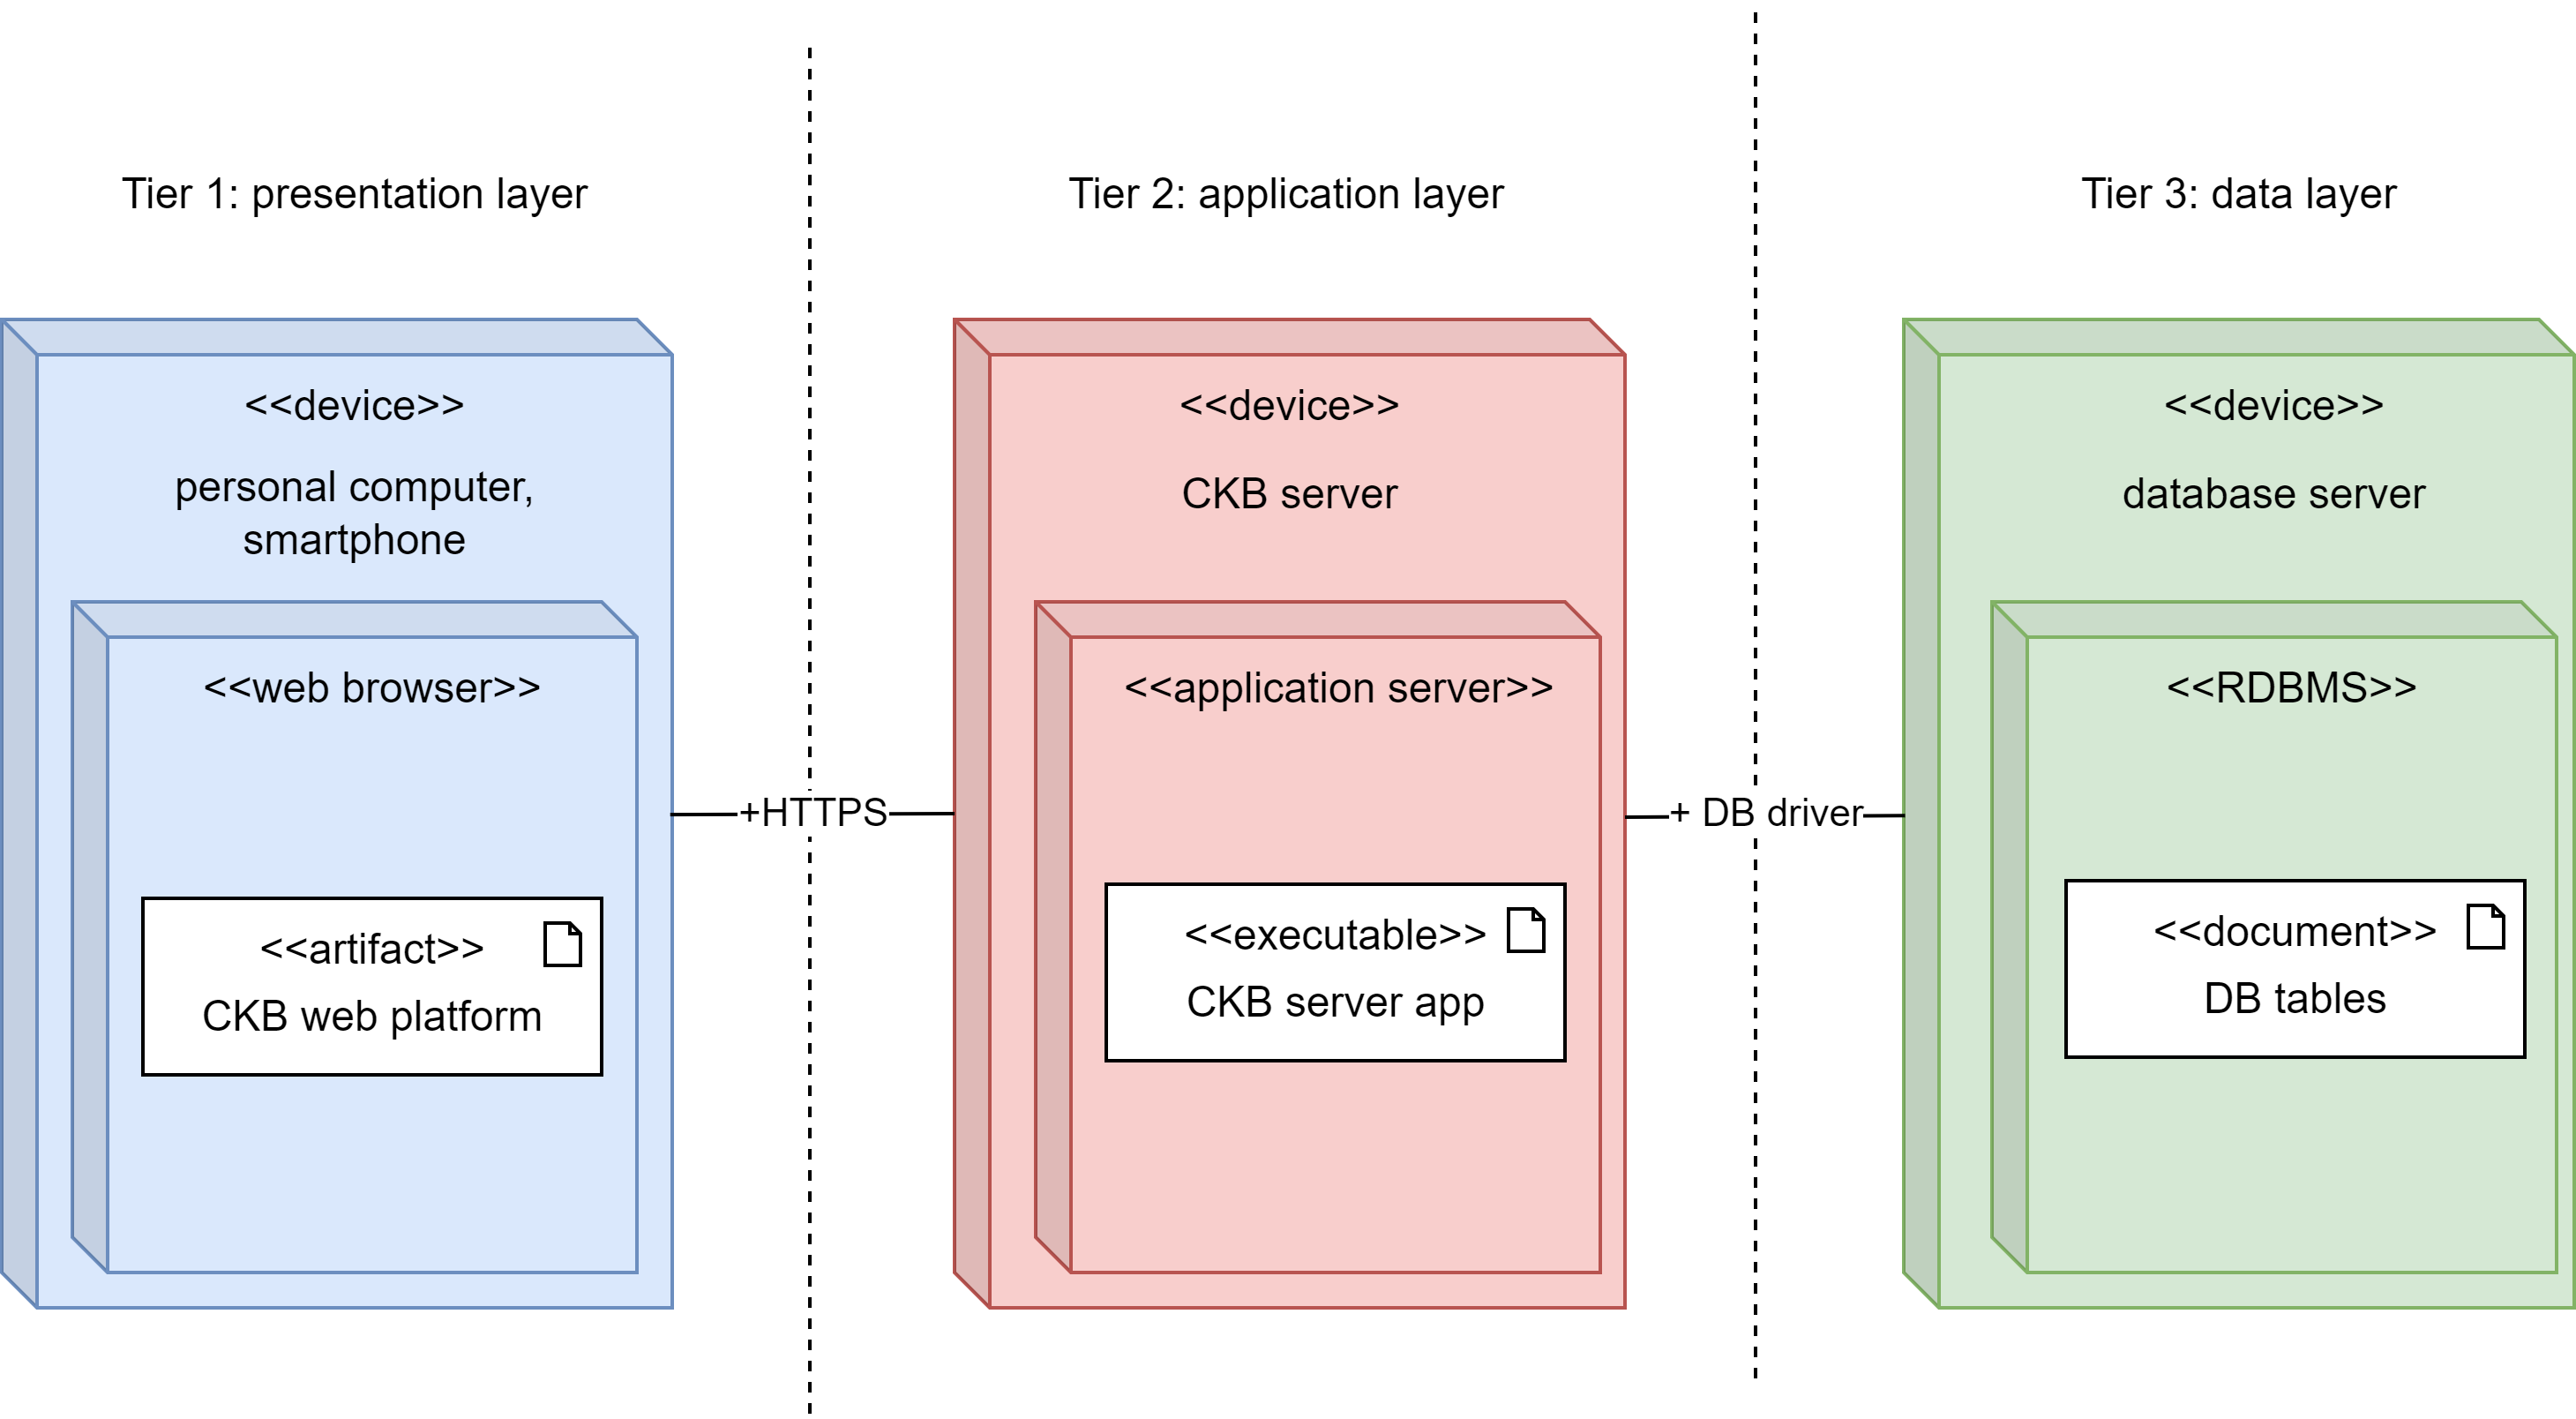
\includegraphics[scale=0.8]{images/deployment.png}
    \caption{Deployment diagram}
    \label{fig:deployment}
\end{figure}
\clearpage

\section{Component interface}
\clearpage

\section{Run-time view}
\clearpage

\section{Selected architectural styles and patterns}
\subsubsection*{Client-Server Architecture}
As previously mentioned in section \ref{sec: overview} the CKB system will be developed based on the client-server architecture. Client and server are two separate objects that communicate over a network: a client makes a request for a service, the server receives this request, process it, and sends back a response. 
\begin{figure}[h]
    \centering 
    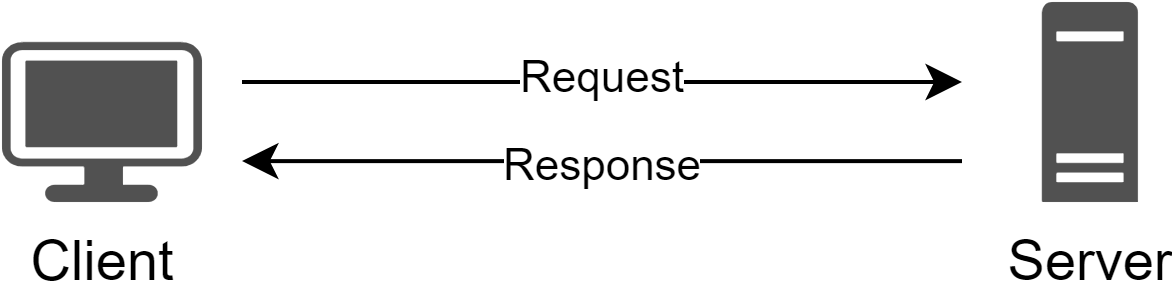
\includegraphics[scale=0.8]{images/CS.png}
    \caption{Client-Server paradigm}
    \label{fig:CS}
\end{figure}

\subsection*{3-tier Architecture}
As previously mentioned in section \ref{sec: overview} and in section \ref{sec: deployment} the CKB system will adopt the three-tier architecture, and for this reason it will be developed in three independent layers (or tiers).

\subsection*{Model View Controller Pattern}
The software will be implemented based on a MVC patter, that divides the program logic into three interconnected parts:
\begin{itemize}
    \item Model: it is the core element of the entire system that directly manage the logic of the CKB platform. 
    \item View: it manages all user interfaces.
    \item Controller: it handles all inputs from the view and manipulates the objects in the model.
\end{itemize}
\begin{figure}[h]
    \centering 
    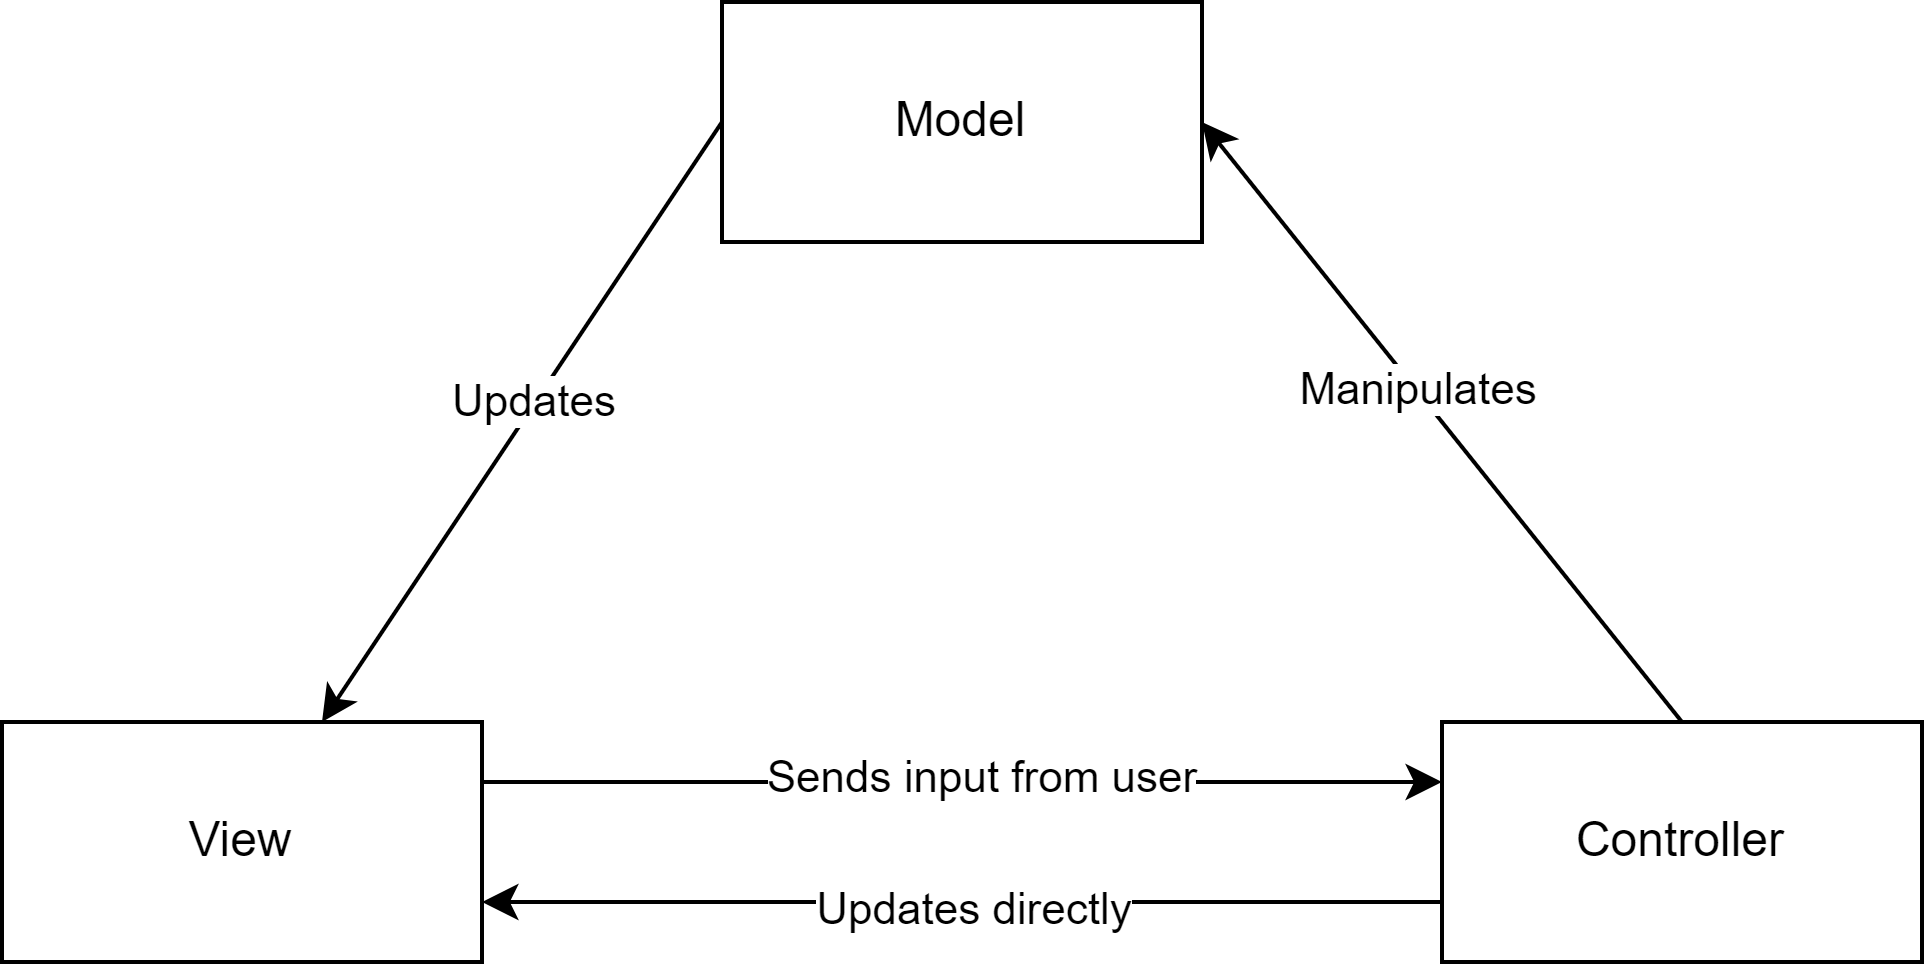
\includegraphics[scale=0.8]{images/MVC.png}
    \caption{Model-View-Controller paradigm}
    \label{fig:MVC}
\end{figure}

\subsection*{Facade pattern}
The dashboard component is implemented using the facade pattern, which hide the system's complexity from the client and offers a more user-friendly interface.
In this way the client communicates only with the dashboard interface, that manages all inputs. The dashboard manager communicates with the appropriate sub-component based on the client request.

\clearpage
\section{Other design decision}
\subsection*{Relational DBMS}
The data layer, as mentioned in section \ref{sec: deployment}, consists of a relational DBMS. A MySQL DBMS will be used since it is an open-source relational database management system (RDBMS). \newline
In figure \ref{fig:DB} shows the database structure. \newline
For clarity, the "password" attribute in the user table is represented, but will be encrypted, and the "studentID" attribute is the same as "username" for a student. 

\begin{figure}[h]
    \centering 
    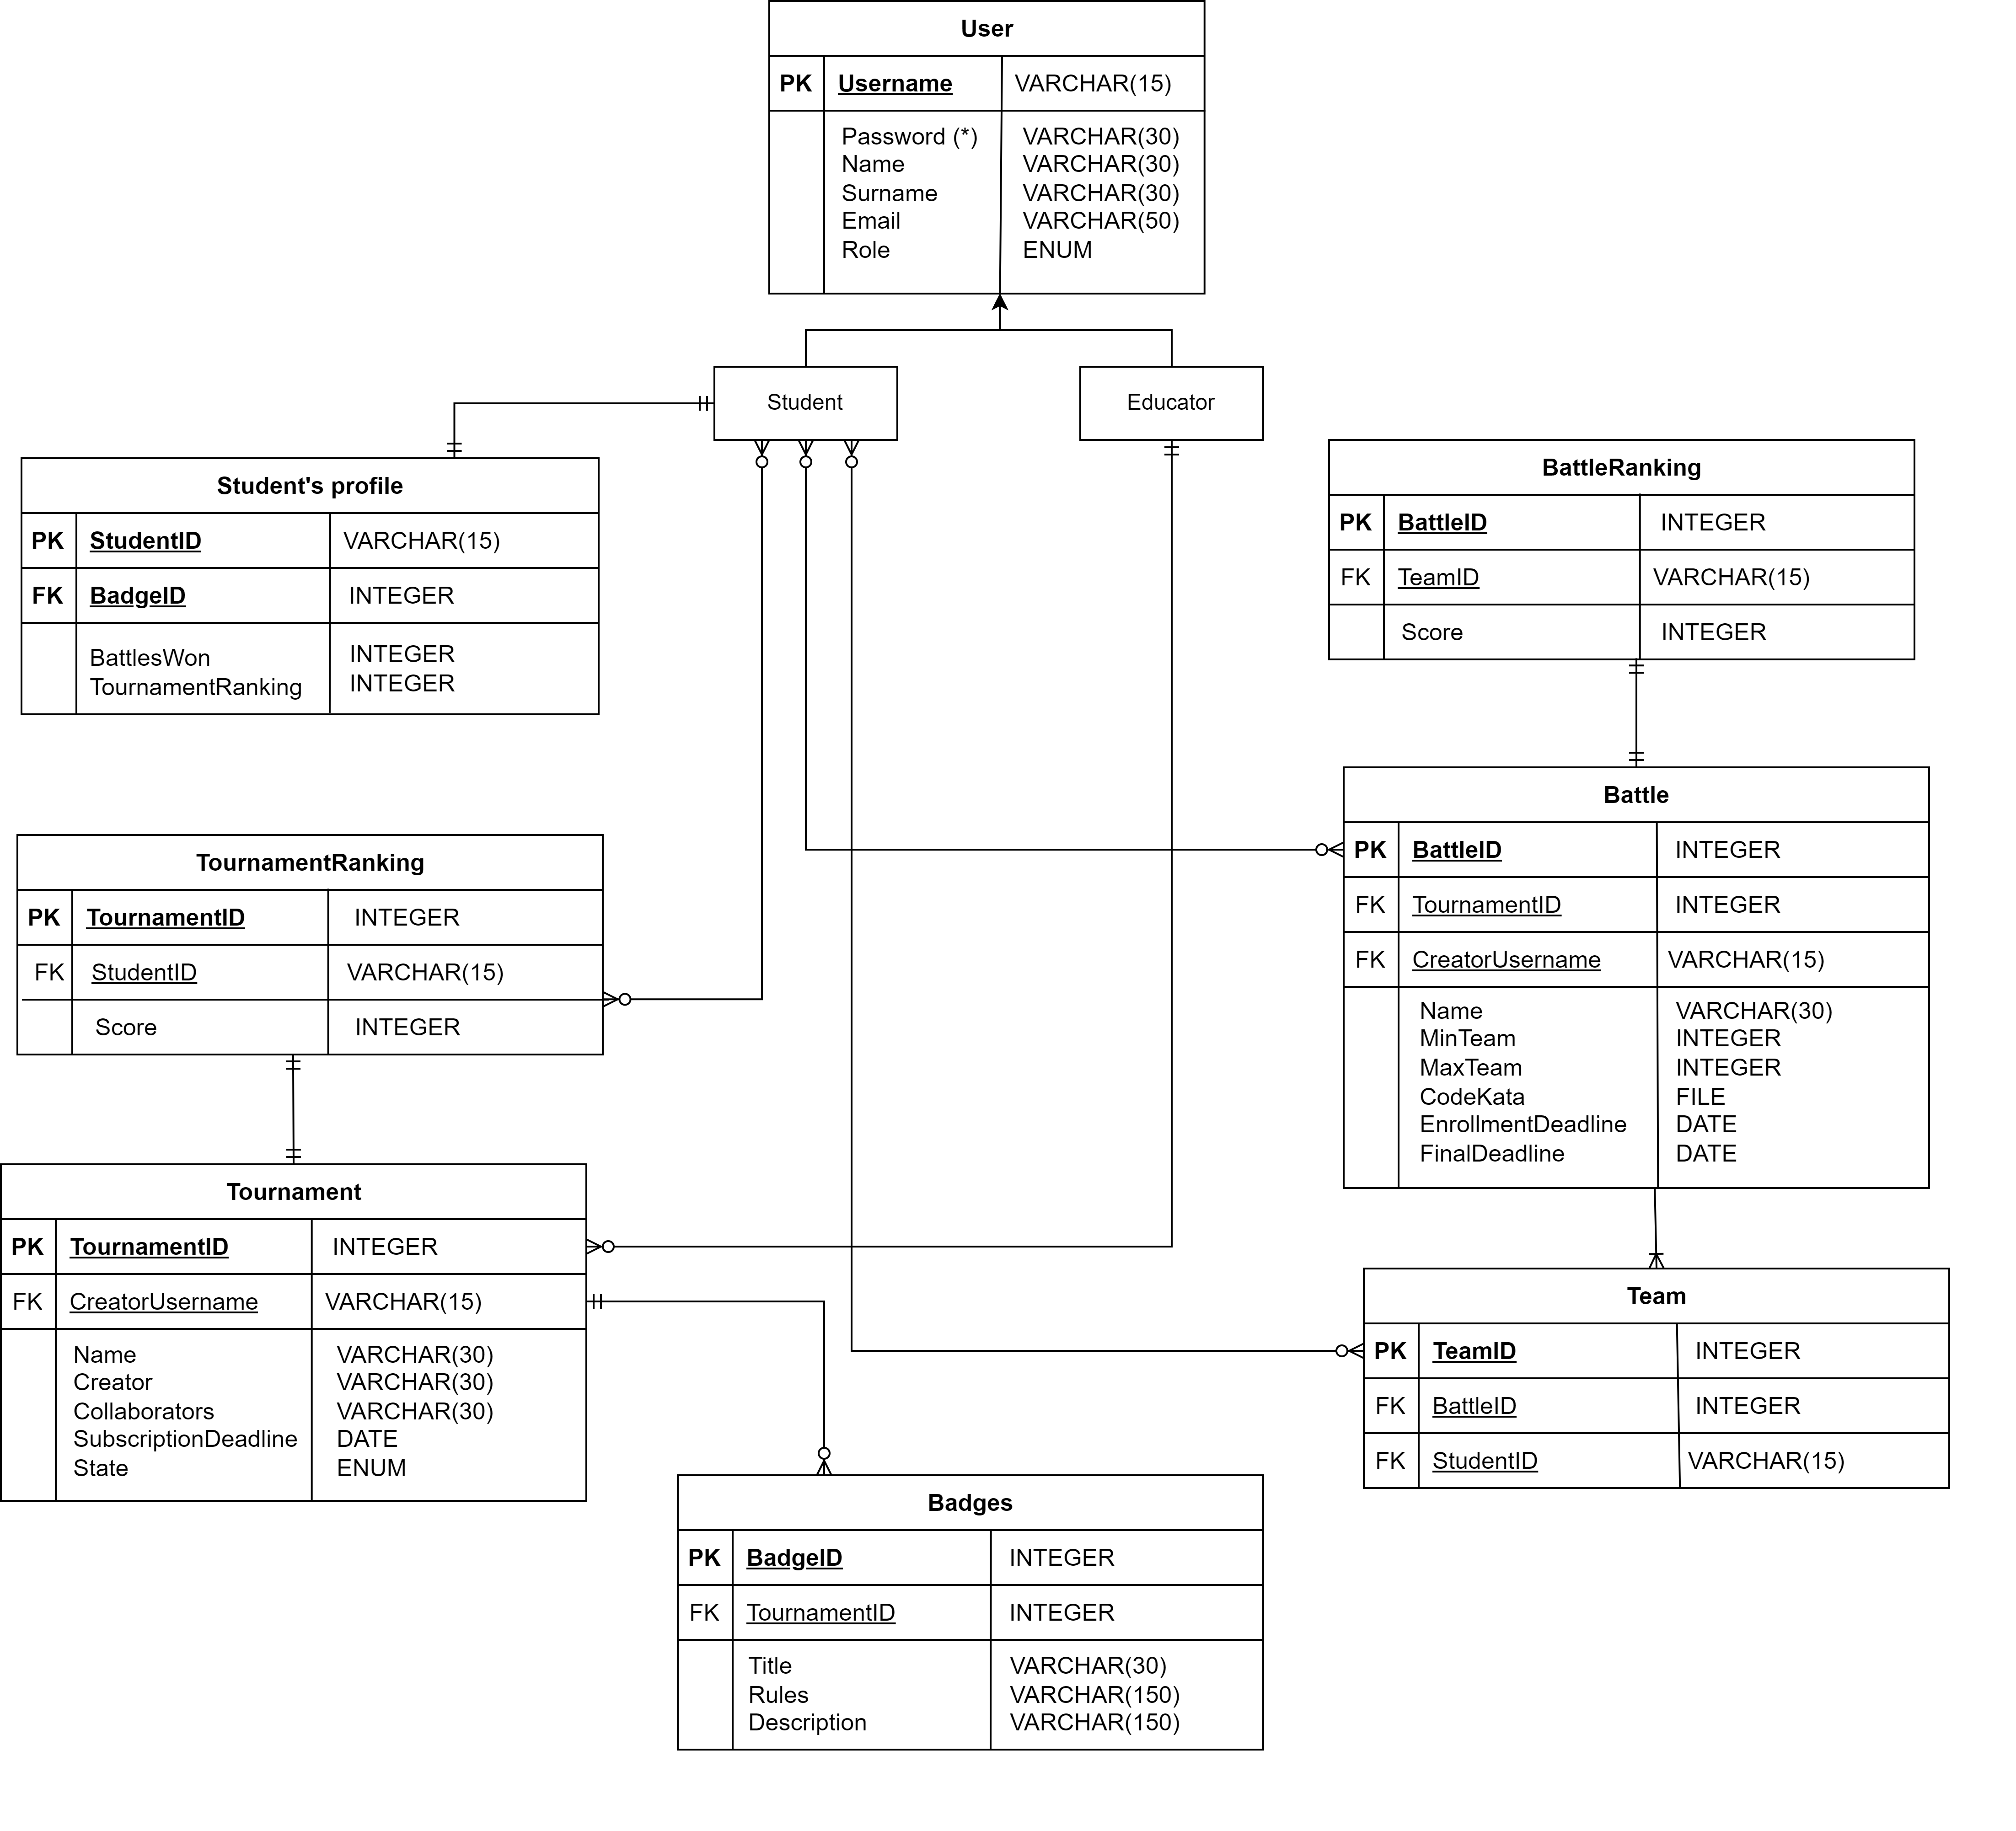
\includegraphics[width=\textwidth]{images/DB.png}
    \caption{Database structure}
    \label{fig:DB}
\end{figure}
